
%(BEGIN_QUESTION)
% Copyright 2006, Tony R. Kuphaldt, released under the Creative Commons Attribution License (v 1.0)
% This means you may do almost anything with this work of mine, so long as you give me proper credit

Dette {\it kromatogrammet} viser separasjon av fem ulike stoffer over tid:

$$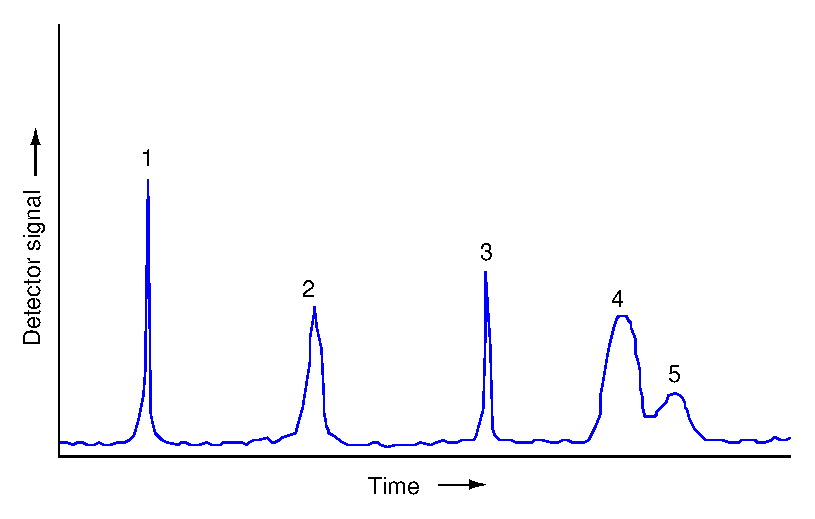
\includegraphics[width=15.5cm]{i00672x01.eps}$$

Legg merke til at komponent 4 og 5 ikke er tydelig skilt i kromatogrammet. Identifiser minst én måte kromatografen kan justeres på for å få tydeligere separasjon (bedre {\it oppløsning}) av de to siste komponentene.

\underbar{file i00672no}
%(END_QUESTION)





%(BEGIN_ANSWER)

\begin{itemize}
\item{} Bruk en tettere stasjonær fase i kolonnen.
\item{} Bruk en stasjonær fase med bedre adsorpsjonsevne (og/eller løselighet).
\item{} Bruk temperatur- eller flow-"programmering" for å senke elueringen av de to siste komponentene slik at separasjonen blir bedre.
\end{itemize}

%(END_ANSWER)





%(BEGIN_NOTES)


%INDEX% Måling, analytisk: kromatografi

%(END_NOTES)
